\documentclass[uplatex,dvipdfmx]{beamer}
\usepackage{graphicx}

\usetheme{Opencampus}

% 好みの色で
\usecolortheme[RGB={0,128,192}]{structure}
%\usecolortheme[RGB={205,173,0}]{structure}
% \usecolortheme[RGB={173,205,0}]{structure}
%\usecolortheme[RGB={30,220,180}]{structure}
%\usecolortheme[RGB={84,255,159}]{structure}
%\usecolortheme[RGB={180,64,169}]{structure}
%\usecolortheme[RGB={255,131,250}]{structure}

\usepackage{booktabs}
\usepackage{colortbl}
\usepackage{pxjahyper} %目次、タイトルバーの文字化け解消
\boldmath

\usepackage[orientation=portrait,size=a1,scale=2]{beamerposter}
% scale の値で文字の大きさを調整できる

\usefonttheme{professionalfonts} 
\renewcommand{\familydefault}{\sfdefault}
\renewcommand{\kanjifamilydefault}{\gtdefault}

\title{\huge タンパク質のアミノ酸配列間距離の評価のための最適なベクトルの割り当て}
\author{土山 啓汰}
\institute{理工学研究科理工学専攻電子情報工学コース1年}
\date{令和4年8月8日}

\begin{document}

\begin{frame}[t]

  \begin{columns}[T,onlytextwidth]
    \column{.48\paperwidth} % 全体の左の列

    \begin{block}{本研究の目標}

      \begin{itemize}
      \item {アミノ酸に三次元ベクトルを割り当て、グラフィカル表現を行う}
      \item {精度を高めるためにアミノ酸のベクトルの割り当て方を検討する}
      \item {各三次元座標群の距離行列を計算し、遺伝子解析同等の系統樹を早く作成する}
      \end{itemize}

    \end{block}




    \begin{block}{検討したアミノ酸の指標・配置}
      
      \begin{itemize}
        \item {指標:疎水性度・等電点・コドン表}
        \item {配置:二重円・左右など}
        \item {現在は三種類の相関のないアミノ酸指標を利用した配置を検討中}
        \item {ポスターでは最も結果が良かった指標・配置を紹介}
      \end{itemize}

    \end{block}

    \begin{block}{ベクトルの割り当て}

      \begin{itemize}
      \item {アミノ酸の疎水性度指標を用いる}
      \end{itemize}

      \begin{table}[H]
        \centering
        \caption{疎水性度表}
        \scalebox{0.8}{
          \begin{tabular}{cc|cc} \hline
          {\small アミノ酸} & {\small 疎水性度} & {\small アミノ酸} & {\small 疎水性度} \\ \hline
          R & -5.10 &G & -0.64 \\[-2mm]
          K & -4.11 &S & -0.50 \\[-2mm]
          Q & -3.68 &W & -0.46 \\[-2mm]
          D & -3.60 &A & 1.10 \\[-2mm]
          N & -3.50 &M & 1.90 \\[-2mm]
          H & -3.20 &C & 2.50 \\[-2mm]
          E & -3.20 &F & 2.80 \\[-2mm]
          P & -1.90 &L & 3.80 \\[-2mm]
          Y & -1.30 &V & 4.20 \\[-2mm]
          T & -0.70 &I & 4.50 \\ \hline
          \end{tabular}
          }
        \end{table}
        
        \begin{itemize}
          \item {アミノ酸を疎水性度の値が小さい順に、内側、外側に10種類ずつ二重円で配置する}
        \end{itemize}

        \begin{figure}[htbp]
          \centering
          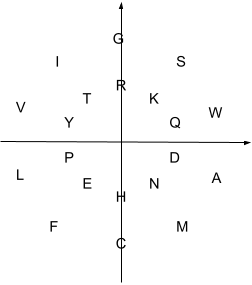
\includegraphics[width=100mm]{pic1.png}
          \caption{アミノ酸のベクトル配置}
        \end{figure}

    \end{block}


    \column{.48\linewidth}
    %% 
    %% 全体の右の列
    %% 

    \begin{block}{三次元座標群のグラフ表示}
      
      \begin{figure}[htbp]
        \centering
        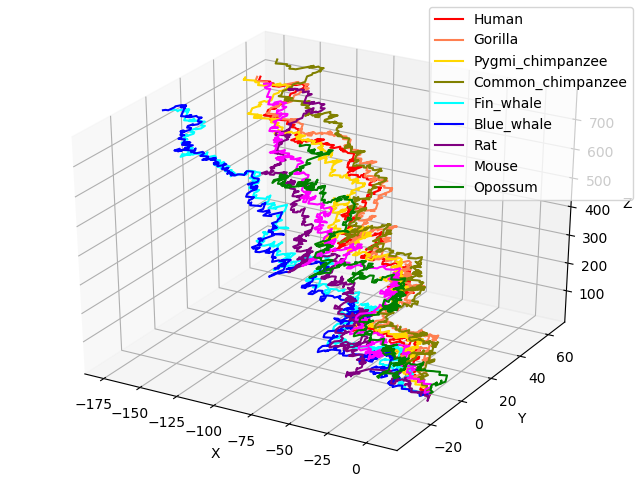
\includegraphics[width=150mm]{pic2.png}
        \caption{三次元座標群のグラフ表示}
      \end{figure}

    \end{block}

    \begin{block}{系統樹の作成}
      
      \begin{itemize}
        \item {各生物種の座標群に対して主成分分析を行い、その第一主成分を元に距離行列\cite{bunken}を計算する}
        \item {距離行列を元に系統樹を作成する}
      \end{itemize}

      \begin{figure}[htbp]
        \centering
        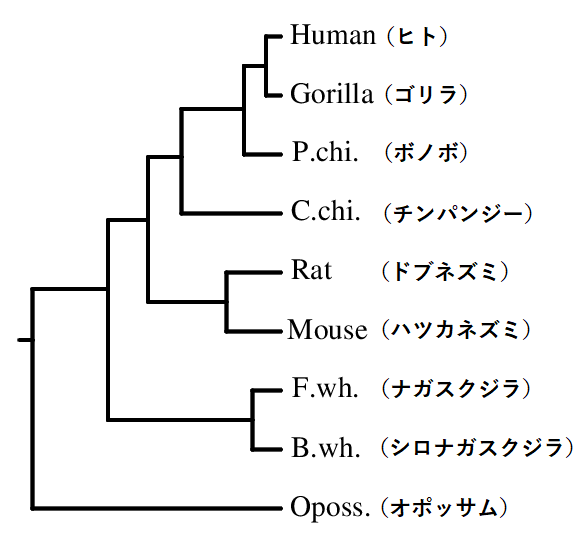
\includegraphics[width=100mm]{pic3.png}
        \caption{作成された系統樹}
      \end{figure}

    \end{block}
    
    \begin{block}{まとめ}
      \begin{itemize}
      \item {近縁種同士のグラフの概形は似ており、直観的に近縁種なのか遠縁種なのか判断できる}
      \item {アミノ酸に割り当てるベクトル配置を複数検討し、より正確な系統樹を作成した}
      \end{itemize}

    \end{block}

    \begin{block}{参考文献}
      % 参考文献のリスト
      \begin{thebibliography}{99}
      \bibitem{bunken} Agata,C ,Dorota,B ,Piotr,W and Tim,C ”20Ddynamic
      representation of protein sequences” Genomics Volume
      107, Issue 1, January 2016, Pages16-23
      \end{thebibliography}
    \end{block}

  \end{columns}

\end{frame}
\end{document}

%%% Local Variables: 
%%% mode: latex
%%% TeX-PDF-mode: t
%%% TeX-master: t
%%% End:
